\documentclass[12pt,a4paper]{article}

\usepackage{fontspec}
\usepackage{polyglossia}
\setdefaultlanguage{greek}
\setotherlanguage{english}

\setmainfont[Script=Greek]{DejaVu Serif}
\setsansfont[Script=Greek]{DejaVu Sans}
\setmonofont[Script=Greek]{DejaVu Sans Mono}
\newfontfamily\greekfonttt[Script=Greek]{DejaVu Sans Mono}

\usepackage[margin=2.5cm]{geometry}
\usepackage{graphicx}
\usepackage{float}
\usepackage{caption}
\usepackage{amsmath}
\usepackage{amssymb}
\usepackage{booktabs}
\usepackage{longtable}
\usepackage{multirow}
\usepackage{array}
\usepackage[hidelinks]{hyperref}
\usepackage{fancyhdr}
\usepackage{enumitem}
\usepackage{parskip}

\pagestyle{fancy}
\fancyhf{}
\rhead{ΑΕΜ: 6931 -- Ρακοβαλής Παύλος}
\lhead{Ανάλυση Δεδομένων 2025--26}
\cfoot{\thepage}

\title{
    \textbf{Ανάλυση Δεδομένων 2025--26}\\[0.3cm]
    \Large 2η Εργασία: Ανάλυση Παλινδρόμησης\\[0.2cm]
    \large Πρόβλεψη Ποιότητας Κρασιού
}
\author{
    Ρακοβαλής Παύλος\\
    ΑΕΜ: 6931
}
\date{\today}

\begin{document}

\maketitle
\thispagestyle{fancy}

%==========================================================================
\section*{Περίληψη}
%==========================================================================

Στην παρούσα εργασία διερευνάται κατά πόσο οι φυσικοχημικές ιδιότητες του κρασιού μπορούν να προβλέψουν τη βαθμολογία ποιότητάς του. Χρησιμοποιούνται 5.274 παρατηρήσεις (τυχαίο δείγμα βάσει ΑΕΜ 6931) με 11 συνεχείς μεταβλητές-προβλέπτες και μεταβλητή απόκρισης τη βαθμολογία ποιότητας (\texttt{quality}). Εφαρμόζονται μέθοδοι απλής και πολλαπλής γραμμικής παλινδρόμησης, πρόσω επιλογή μεταβλητών, πολυωνυμική παλινδρόμηση και διαγνωστικοί έλεγχοι. Το βέλτιστο γραμμικό μοντέλο εξηγεί περίπου το 27,7\% της μεταβλητότητας, με σημαντικότερους προβλέπτες το αλκοόλ, την πτητική οξύτητα και τα θειικά. Ο διαγνωστικός έλεγχος αποκαλύπτει παραβιάσεις βασικών υποθέσεων, υποδεικνύοντας ότι εναλλακτικές μέθοδοι (τακτική λογιστική παλινδρόμηση, αλγόριθμοι μηχανικής μάθησης) θα ήταν καταλληλότερες.

\tableofcontents
\newpage

%==========================================================================
\section{Εισαγωγή}
%==========================================================================

\subsection{Σκοπός}

Σκοπός της εργασίας είναι η διερεύνηση της σχέσης μεταξύ των φυσικοχημικών χαρακτηριστικών του κρασιού και της βαθμολογίας ποιότητάς του, μέσω τεχνικών γραμμικής παλινδρόμησης.

\subsection{Δεδομένα}

Χρησιμοποιούνται τα καθαρισμένα δεδομένα της 1ης εργασίας:
\begin{itemize}[nosep]
    \item \textbf{Μεταβλητή απόκρισης} ($Y$): \texttt{quality} -- ακέραιες τιμές 3--9
    \item \textbf{Προβλέπτες} ($X_1, \ldots, X_{11}$): \begin{english}fixed acidity, volatile acidity, citric acid, residual sugar, chlorides, free sulfur dioxide, total sulfur dioxide, density, pH, sulphates, alcohol\end{english}
    \item \textbf{Παρατηρήσεις}: $n = 5.274$
\end{itemize}

%==========================================================================
\section{Απλή Γραμμική Παλινδρόμηση (Υποερώτημα 1)}
%==========================================================================

\subsection{Μεθοδολογία}

Προσαρμόστηκαν 11 μοντέλα απλής γραμμικής παλινδρόμησης της μορφής:
\begin{equation}
    Y = \beta_0 + \beta_1 X_j + \varepsilon, \quad j = 1, \ldots, 11
\end{equation}
με τη μέθοδο ελαχίστων τετραγώνων (OLS). Για κάθε μοντέλο εκτιμήθηκαν οι συντελεστές $\hat{\beta}_0$, $\hat{\beta}_1$ και ελέγχθηκε η μηδενική υπόθεση $H_0: \beta_1 = 0$ έναντι $H_1: \beta_1 \neq 0$ σε επίπεδο σημαντικότητας $\alpha = 0.05$.

\subsection{Αποτελέσματα}

\begin{table}[H]
\centering
\caption{Αποτελέσματα απλής γραμμικής παλινδρόμησης (ταξινομημένα κατά $R^2$)}
\label{tab:simple_regression}
\small
\begin{tabular}{lrrrrl}
\toprule
\textbf{Μεταβλητή} & $\hat{\beta}_1$ & \textbf{t-stat} & \textbf{p-value} & $R^2$ & \textbf{Σημαντ.} \\
\midrule
\begin{english}alcohol\end{english}              &  $+0.343$   & $35.13$   & $\approx 0$           & 0.1897 & Ναι \\
\begin{english}density\end{english}              & $-94.21$    & $-23.40$  & $2.6 \times 10^{-115}$ & 0.0941 & Ναι \\
\begin{english}volatile acidity\end{english}     & $-1.386$    & $-19.08$  & $1.6 \times 10^{-78}$  & 0.0646 & Ναι \\
\begin{english}chlorides\end{english}            & $-5.078$    & $-15.09$  & $2.2 \times 10^{-50}$  & 0.0414 & Ναι \\
\begin{english}citric acid\end{english}          &  $+0.566$   & $6.86$    & $7.5 \times 10^{-12}$  & 0.0089 & Ναι \\
\begin{english}fixed acidity\end{english}        & $-0.052$    & $-5.24$   & $1.7 \times 10^{-7}$   & 0.0052 & Ναι \\
\begin{english}residual sugar\end{english}       & $-0.010$    & $-3.88$   & $1.0 \times 10^{-4}$   & 0.0029 & Ναι \\
\begin{english}total sulfur dioxide\end{english} & $-0.001$    & $-3.79$   & $1.5 \times 10^{-4}$   & 0.0027 & Ναι \\
\begin{english}free sulfur dioxide\end{english}  &  $+0.003$   & $3.79$    & $1.6 \times 10^{-4}$   & 0.0027 & Ναι \\
\begin{english}sulphates\end{english}            &  $+0.253$   & $3.09$    & $2.0 \times 10^{-3}$   & 0.0018 & Ναι \\
\begin{english}pH\end{english}                   &  $+0.175$   & $2.19$    & $2.8 \times 10^{-2}$   & 0.0009 & Ναι \\
\bottomrule
\end{tabular}
\end{table}

Η $H_0: \beta_1 = 0$ \textbf{απορρίπτεται} και για τις 11 μεταβλητές ($p < 0.05$). Ο ισχυρότερος μεμονωμένος προβλέπτης είναι το αλκοόλ ($R^2 = 0.19$), ακολουθούμενο από την πυκνότητα ($R^2 = 0.09$) και την πτητική οξύτητα ($R^2 = 0.06$). Ωστόσο, κανένας μεμονωμένος προβλέπτης δεν εξηγεί ικανοποιητικό ποσοστό της μεταβλητότητας.

\begin{figure}[H]
    \centering
    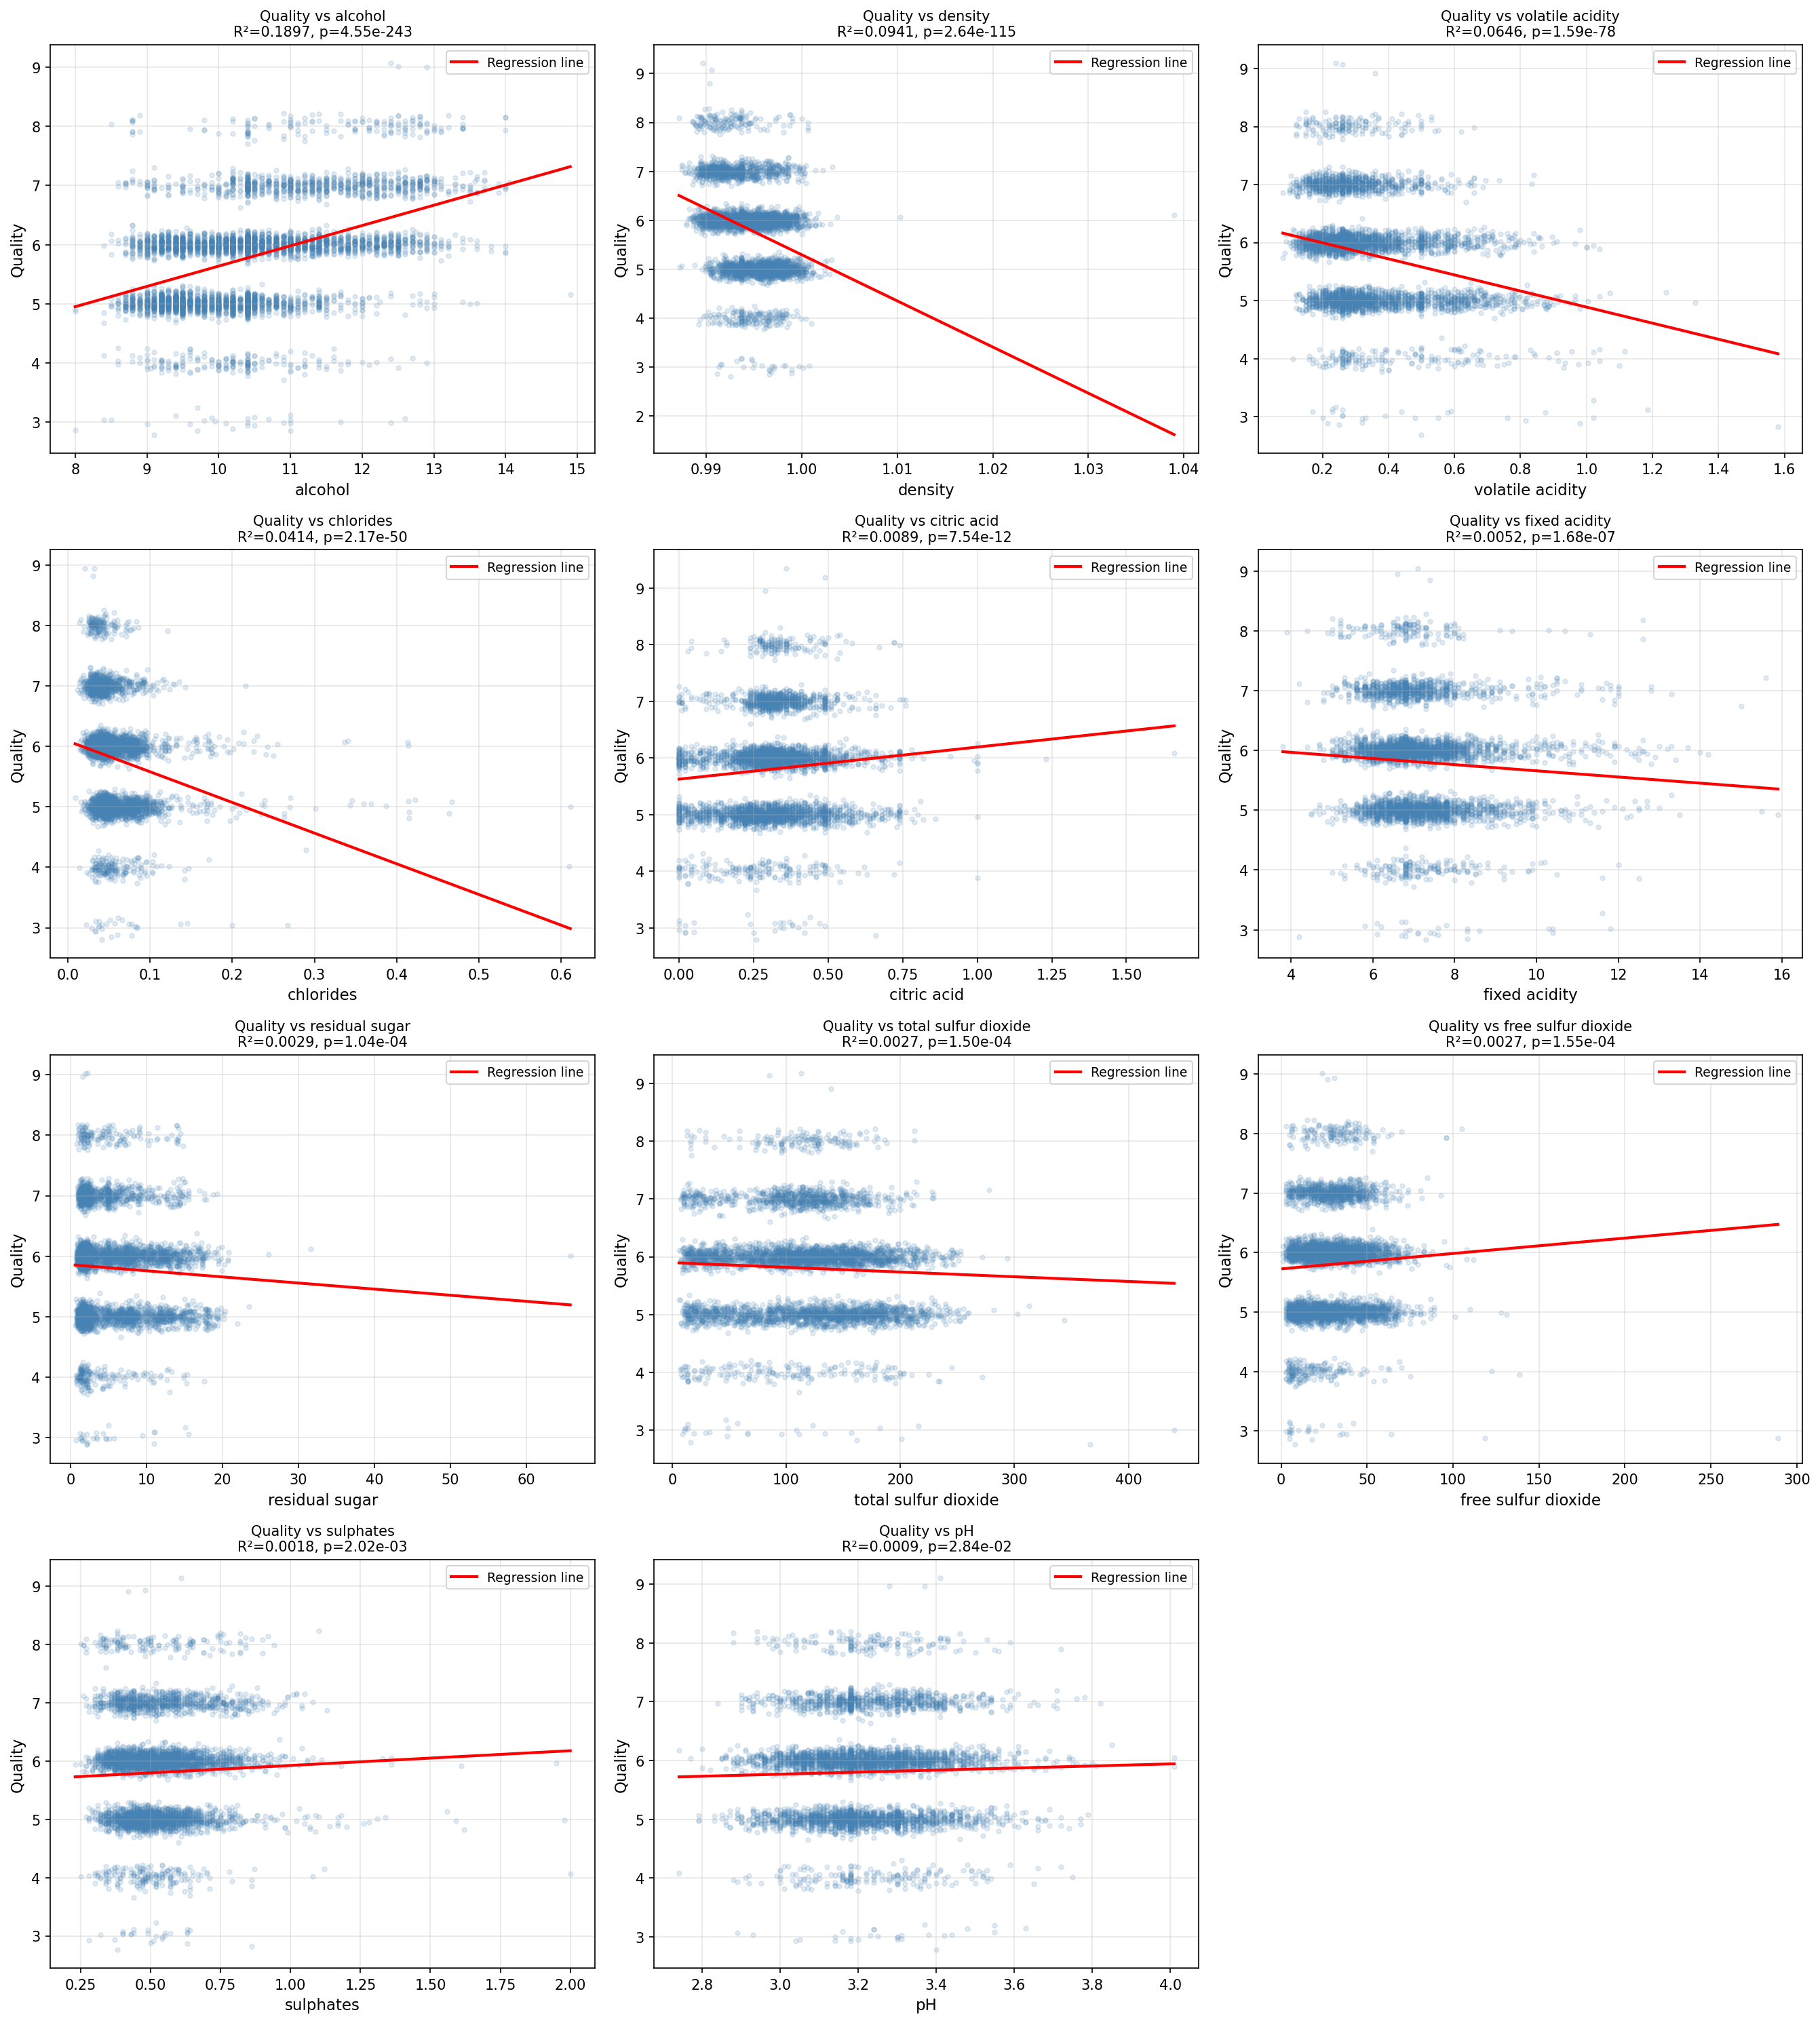
\includegraphics[width=\textwidth]{scatter_plots_significant.png}
    \caption{Διαγράμματα διασποράς (με ευθεία παλινδρόμησης) για τους σημαντικούς μεμονωμένους προβλέπτες.}
    \label{fig:scatter}
\end{figure}

%==========================================================================
\section{Πολλαπλή Γραμμική Παλινδρόμηση (Υποερώτημα 2)}
%==========================================================================

\subsection{Μεθοδολογία}

Προσαρμόστηκε μοντέλο πολλαπλής γραμμικής παλινδρόμησης με όλες τις 11 μεταβλητές:
\begin{equation}
    Y = \beta_0 + \beta_1 X_1 + \beta_2 X_2 + \cdots + \beta_{11} X_{11} + \varepsilon
\end{equation}

Ελέγχθηκε πρώτα η συνολική σημαντικότητα μέσω F-ελέγχου ($H_0: \beta_1 = \beta_2 = \cdots = \beta_{11} = 0$) και στη συνέχεια η σημαντικότητα κάθε μεταβλητής μέσω μερικού t-ελέγχου ($H_0: \beta_j = 0$, $j = 1, \ldots, 11$).

\subsection{Αποτελέσματα}

\textbf{Συνολική αξιολόγηση μοντέλου:}
\begin{itemize}[nosep]
    \item $R^2 = 0.2771$, $R^2_{adj} = 0.2756$
    \item $F(11, 5262) = 183.41$, $p \approx 0$ $\Rightarrow$ απόρριψη $H_0$ -- το μοντέλο είναι συνολικά σημαντικό
    \item $AIC = 11880.85$, $BIC = 11959.70$
\end{itemize}

\begin{table}[H]
\centering
\caption{Συντελεστές πολλαπλής γραμμικής παλινδρόμησης}
\label{tab:multiple_regression}
\small
\begin{tabular}{lrrrrl}
\toprule
\textbf{Μεταβλητή} & $\hat{\beta}_j$ & \textbf{SE} & \textbf{t-stat} & \textbf{p-value} & $H_0: \beta_j=0$ \\
\midrule
Σταθερά            &   $44.231$   & 8.847  &  $5.00$   & $5.9 \times 10^{-7}$  & Απορρίπτεται \\
\begin{english}fixed acidity\end{english}        &   $0.042$    & 0.014  &  $3.03$   & $2.5 \times 10^{-3}$  & Απορρίπτεται \\
\begin{english}volatile acidity\end{english}     &  $-1.250$    & 0.087  & $-14.39$  & $4.4 \times 10^{-46}$ & Απορρίπτεται \\
\begin{english}citric acid\end{english}          &   $0.131$    & 0.088  &  $1.49$   & $1.4 \times 10^{-1}$  & \textbf{Δεν απορρ.} \\
\begin{english}residual sugar\end{english}       &   $0.029$    & 0.004  &  $7.09$   & $1.5 \times 10^{-12}$ & Απορρίπτεται \\
\begin{english}chlorides\end{english}            &  $-1.354$    & 0.369  & $-3.67$   & $2.4 \times 10^{-4}$  & Απορρίπτεται \\
\begin{english}free sulfur dioxide\end{english}  &   $0.007$    & 0.001  &  $8.26$   & $1.8 \times 10^{-16}$ & Απορρίπτεται \\
\begin{english}total sulfur dioxide\end{english} &  $-0.003$    & 0.0003 & $-9.84$   & $1.2 \times 10^{-22}$ & Απορρίπτεται \\
\begin{english}density\end{english}              & $-43.092$    & 9.006  & $-4.79$   & $1.8 \times 10^{-6}$  & Απορρίπτεται \\
\begin{english}pH\end{english}                   &   $0.408$    & 0.088  &  $4.62$   & $4.0 \times 10^{-6}$  & Απορρίπτεται \\
\begin{english}sulphates\end{english}            &   $0.773$    & 0.083  &  $9.34$   & $1.4 \times 10^{-20}$ & Απορρίπτεται \\
\begin{english}alcohol\end{english}              &   $0.272$    & 0.015  & $18.51$   & $4.0 \times 10^{-74}$ & Απορρίπτεται \\
\bottomrule
\end{tabular}
\end{table}

Η $H_0: \beta_j = 0$ απορρίπτεται για \textbf{10 από τις 11} μεταβλητές. Μοναδική εξαίρεση αποτελεί το \begin{english}citric acid\end{english} ($p = 0.138$), η πληροφορία του οποίου αλληλοεπικαλύπτεται με τις υπόλοιπες μεταβλητές οξύτητας (πολυσυγγραμμικότητα). Αξίζει να σημειωθεί ότι στην απλή παλινδρόμηση η ίδια μεταβλητή ήταν στατιστικά σημαντική ($p = 7.5 \times 10^{-12}$).

Επιπλέον, η μεταβλητή \begin{english}residual sugar\end{english} αλλάζει πρόσημο (από $-0.010$ στην απλή σε $+0.029$ στην πολλαπλή παλινδρόμηση), φαινόμενο γνωστό ως παράδοξο Simpson.

%==========================================================================
\section{Πρόσω Επιλογή Μεταβλητών (Υποερώτημα 3)}
%==========================================================================

\subsection{Μεθοδολογία}

Εφαρμόστηκε η μέθοδος πρόσω επιλογής (\begin{english}forward selection\end{english}) με κριτήριο εισόδου $p < 0.05$. Σε κάθε βήμα, προστίθεται η μεταβλητή με τη μικρότερη p-value (δεδομένων των ήδη εισηγμένων), εφόσον αυτή πληροί το κριτήριο. Η διαδικασία τερματίζεται όταν καμία εναπομείνασα μεταβλητή δεν είναι σημαντική.

\subsection{Αποτελέσματα}

\begin{table}[H]
\centering
\caption{Βήματα πρόσω επιλογής μεταβλητών}
\label{tab:forward}
\small
\begin{tabular}{clcccc}
\toprule
\textbf{Βήμα} & \textbf{Μεταβλητή} & \textbf{p-value} & $R^2_{adj}$ & $\Delta R^2_{adj}$ & \textbf{AIC} \\
\midrule
1  & \begin{english}alcohol\end{english}              & $4.5 \times 10^{-243}$ & 0.1895 & $+0.190$ & 12463 \\
2  & \begin{english}volatile acidity\end{english}     & $1.1 \times 10^{-79}$  & 0.2425 & $+0.053$ & 12108 \\
3  & \begin{english}sulphates\end{english}            & $2.1 \times 10^{-18}$  & 0.2533 & $+0.011$ & 12033 \\
4  & \begin{english}free sulfur dioxide\end{english}  & $2.6 \times 10^{-6}$   & 0.2563 & $+0.003$ & 12013 \\
5  & \begin{english}total sulfur dioxide\end{english} & $5.6 \times 10^{-16}$  & 0.2653 & $+0.009$ & 11950 \\
6  & \begin{english}residual sugar\end{english}       & $8.8 \times 10^{-8}$   & 0.2692 & $+0.004$ & 11923 \\
7  & \begin{english}chlorides\end{english}            & $6.7 \times 10^{-6}$   & 0.2718 & $+0.003$ & 11905 \\
8  & \begin{english}density\end{english}              & $6.0 \times 10^{-3}$   & 0.2727 & $+0.001$ & 11899 \\
9  & \begin{english}pH\end{english}                   & $2.5 \times 10^{-3}$   & 0.2739 & $+0.001$ & 11892 \\
10 & \begin{english}fixed acidity\end{english}        & $3.7 \times 10^{-4}$   & 0.2755 & $+0.002$ & 11881 \\
\midrule
11 & \begin{english}citric acid\end{english} (απόρριψη) & $0.138$              & --     & --       & --    \\
\bottomrule
\end{tabular}
\end{table}

\begin{figure}[H]
    \centering
    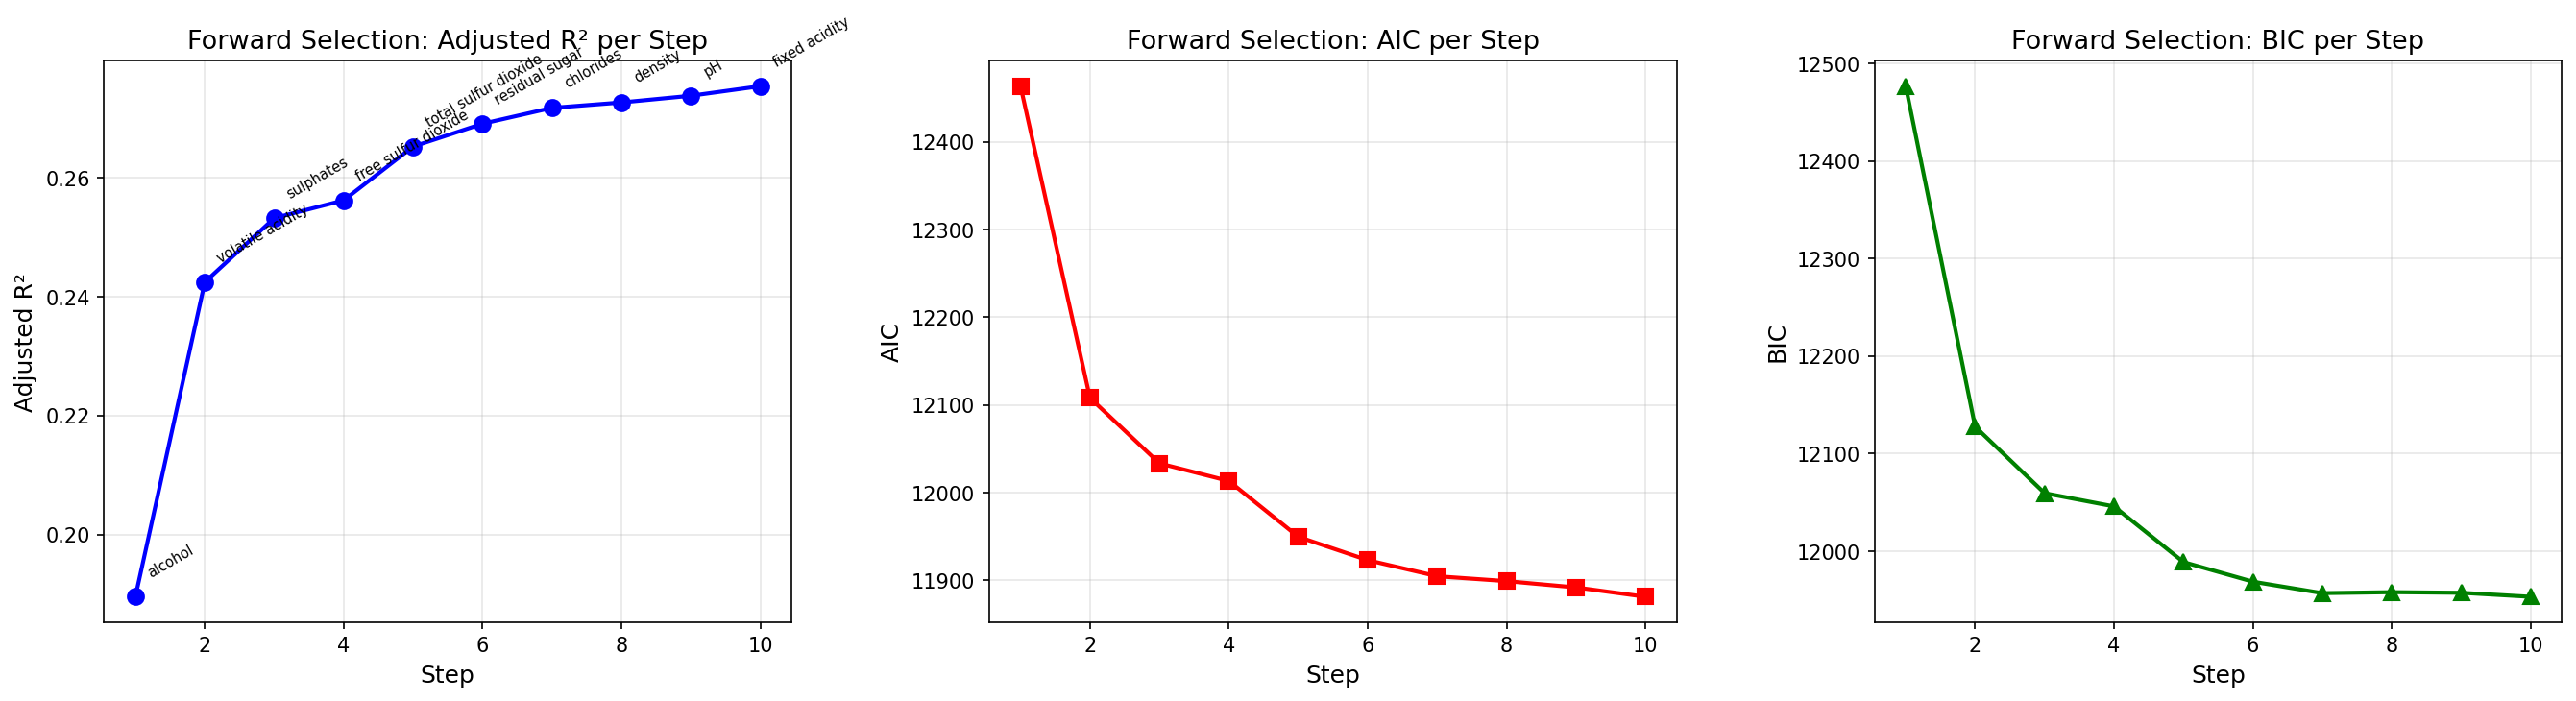
\includegraphics[width=\textwidth]{forward_selection_progression.png}
    \caption{Εξέλιξη $R^2_{adj}$, AIC και BIC κατά τα βήματα της πρόσω επιλογής.}
    \label{fig:forward}
\end{figure}

Η πρόσω επιλογή επέλεξε \textbf{10 από τις 11} μεταβλητές, αποκλείοντας το \begin{english}citric acid\end{english} -- σε συμφωνία με τα αποτελέσματα του Υποερωτήματος 2. Το τελικό μοντέλο ($R^2_{adj} = 0.2755$) είναι ουσιαστικά ισοδύναμο με το πλήρες μοντέλο 11 μεταβλητών ($R^2_{adj} = 0.2756$).

Αξιοσημείωτη είναι η φθίνουσα οριακή απόδοση: οι 3 πρώτες μεταβλητές (\begin{english}alcohol, volatile acidity, sulphates\end{english}) εξηγούν $R^2_{adj} = 0.253$, δηλαδή το 92\% της ερμηνευτικής ικανότητας του πλήρους μοντέλου, ενώ οι υπόλοιπες 7 προσθέτουν μόλις $+0.022$.

%==========================================================================
\section{Πολυωνυμική Παλινδρόμηση (Υποερώτημα 4)}
%==========================================================================

\subsection{Μεθοδολογία}

Για τις μεταβλητές \begin{english}residual sugar, chlorides\end{english} και \begin{english}alcohol\end{english} προσαρμόστηκαν μοντέλα πολυωνυμικής παλινδρόμησης βαθμού 1, 2 και 3:
\begin{equation}
    Y = \beta_0 + \beta_1 X + \beta_2 X^2 + \beta_3 X^3 + \varepsilon
\end{equation}

Η σημαντικότητα των ανώτερων όρων ($\beta_2$, $\beta_3$) αξιολογήθηκε μέσω t-ελέγχων, ενώ η σύγκριση μοντέλων έγινε μέσω $R^2_{adj}$, AIC και BIC.

\subsection{Αποτελέσματα}

\begin{table}[H]
\centering
\caption{Σύγκριση γραμμικών, τετραγωνικών και κυβικών μοντέλων}
\label{tab:polynomial}
\small
\begin{tabular}{llrrrr}
\toprule
\textbf{Μεταβλητή} & \textbf{Μοντέλο} & $R^2$ & $R^2_{adj}$ & \textbf{AIC} & \textbf{p-value (ανωτ. όρος)} \\
\midrule
\multirow{3}{*}{\begin{english}residual sugar\end{english}}
    & Γραμμικό     & 0.0029 & 0.0027 & 13557 & -- \\
    & Τετραγωνικό  & 0.0031 & 0.0027 & 13558 & 0.297 (ΜΣ) \\
    & Κυβικό       & 0.0072 & 0.0066 & 13539 & $3.0 \times 10^{-6}$ \\
\midrule
\multirow{3}{*}{\begin{english}chlorides\end{english}}
    & Γραμμικό     & 0.0414 & 0.0412 & 13350 & -- \\
    & Τετραγωνικό  & 0.0583 & 0.0579 & 13258 & $3.9 \times 10^{-22}$ \\
    & Κυβικό       & 0.0708 & 0.0702 & 13190 & $4.9 \times 10^{-17}$ \\
\midrule
\multirow{3}{*}{\begin{english}alcohol\end{english}}
    & Γραμμικό     & 0.1897 & 0.1895 & 12463 & -- \\
    & Τετραγωνικό  & 0.1903 & 0.1900 & 12461 & 0.046 \\
    & Κυβικό       & 0.1947 & 0.1943 & 12434 & $6.6 \times 10^{-8}$ \\
\bottomrule
\end{tabular}
\end{table}

\begin{figure}[H]
    \centering
    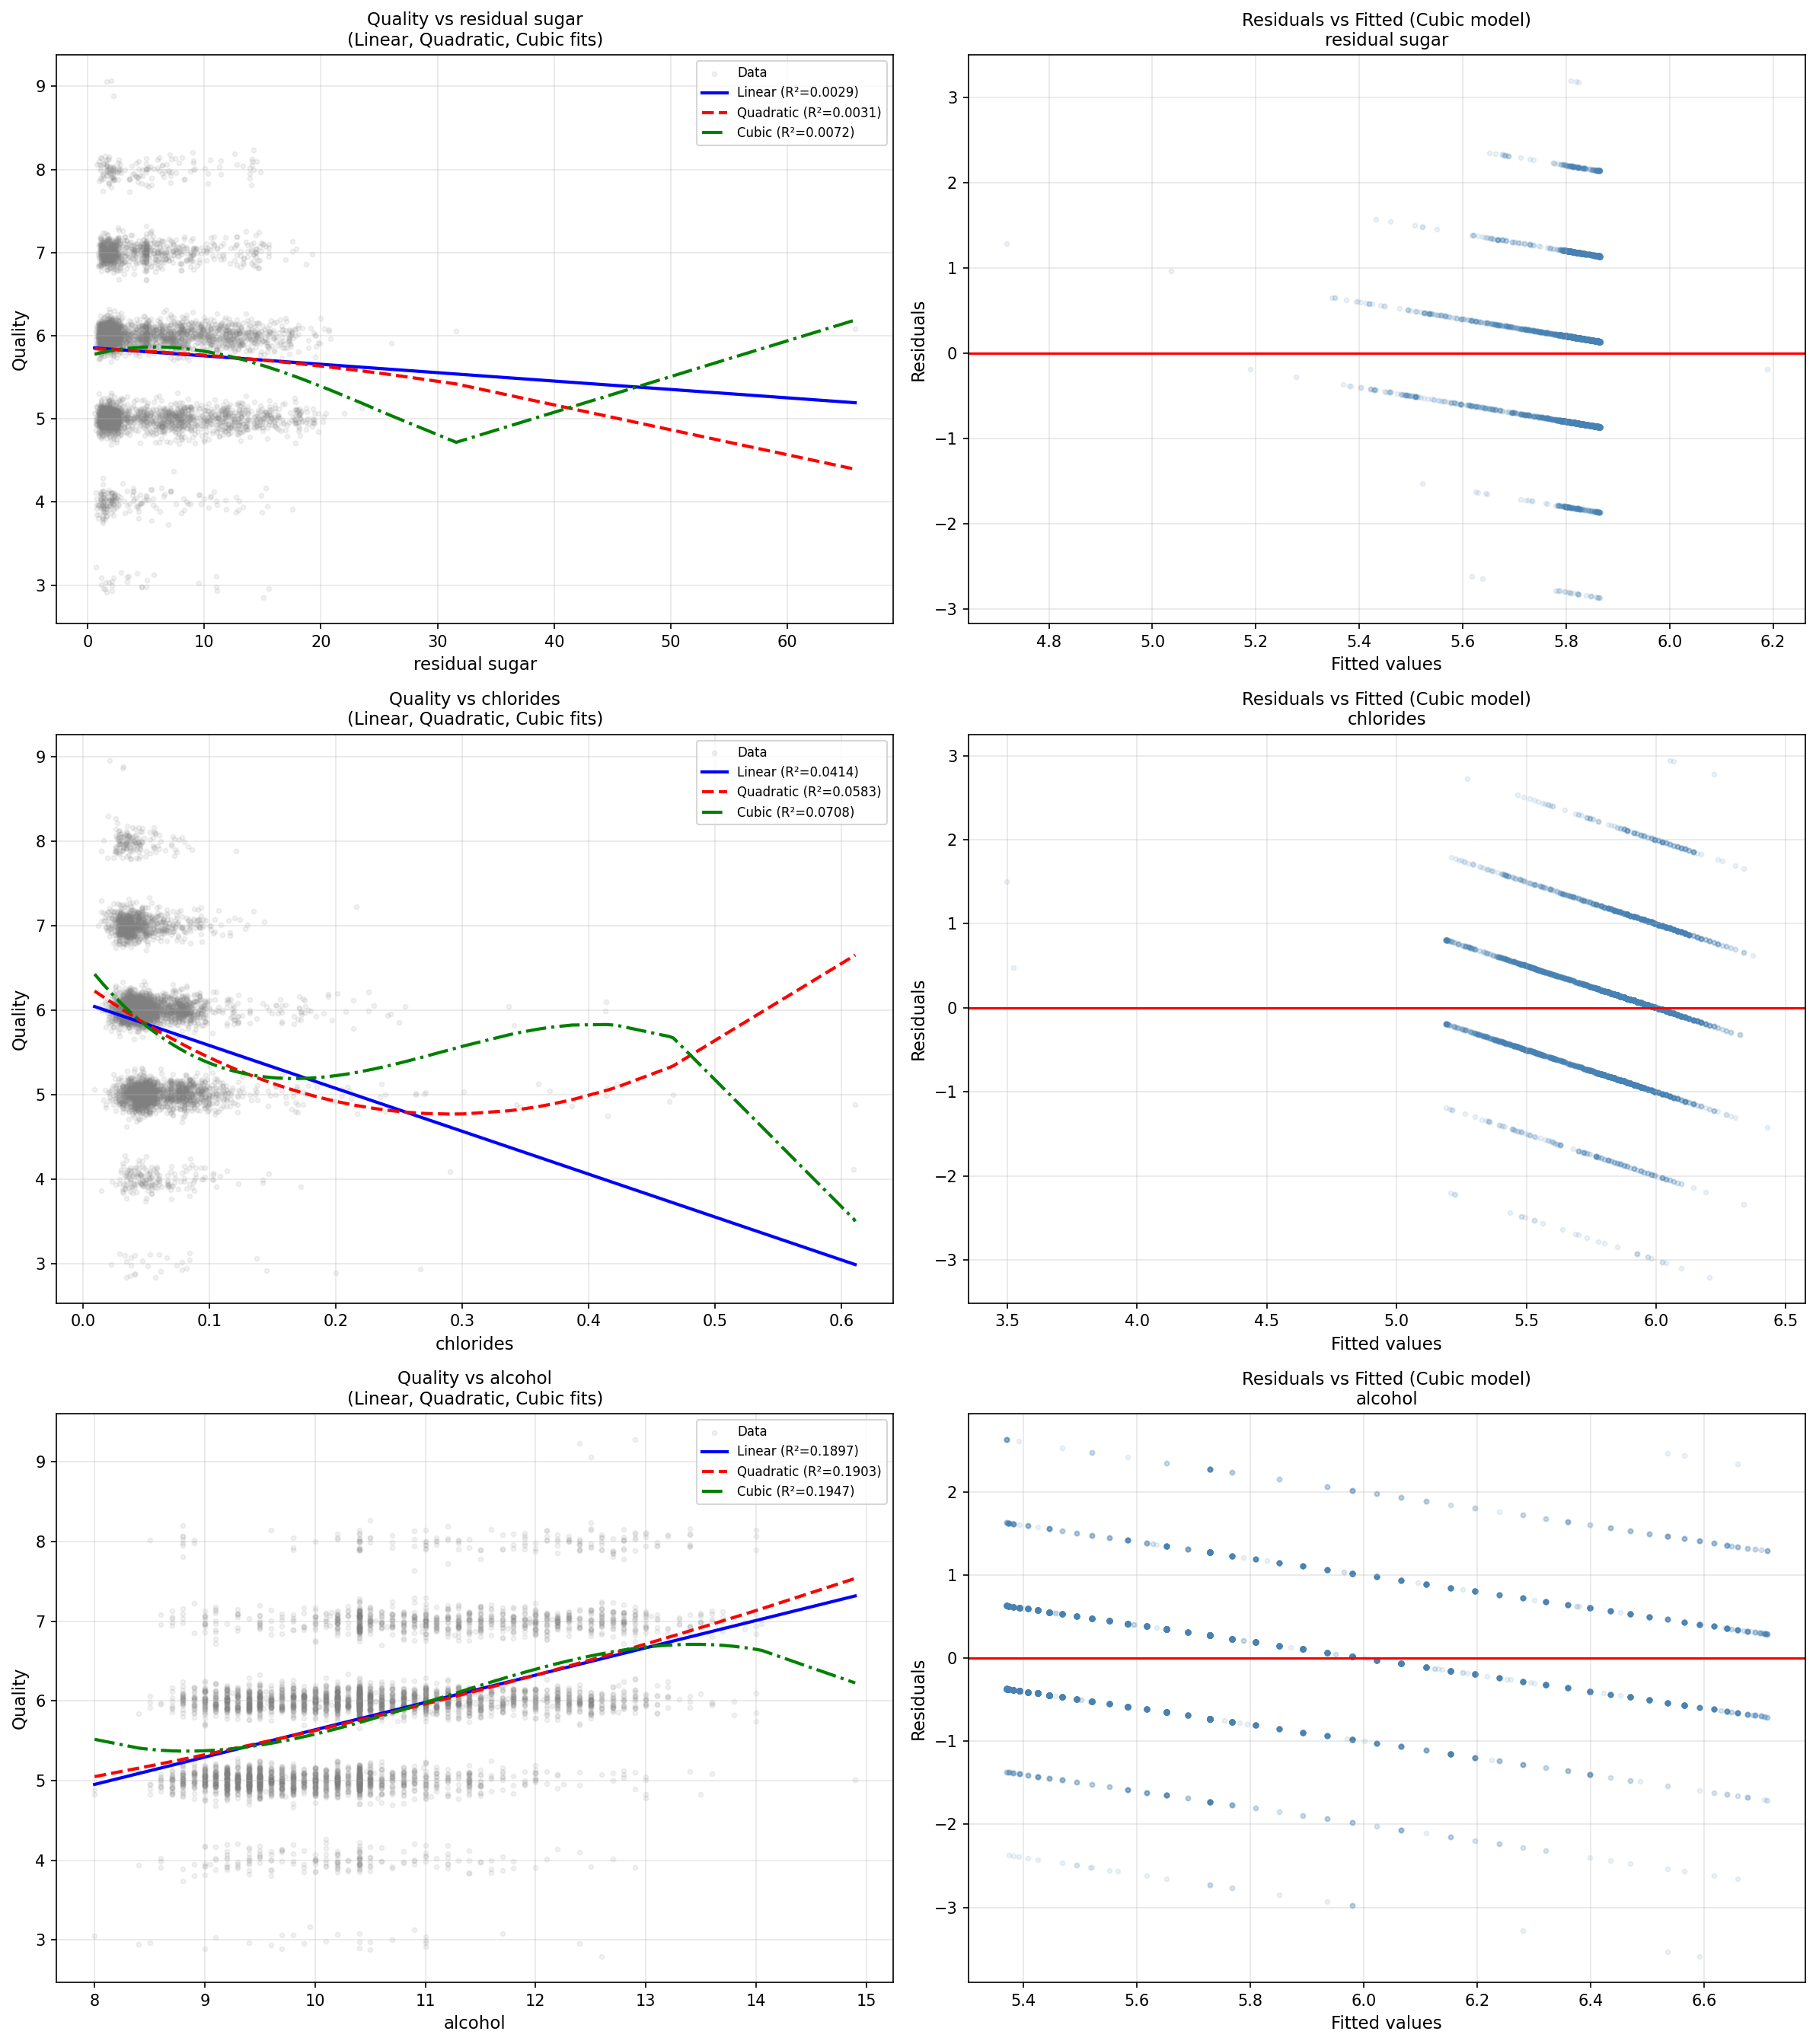
\includegraphics[width=\textwidth]{polynomial_regression.png}
    \caption{Πολυωνυμική παλινδρόμηση: καμπύλες προσαρμογής (αριστερά) και υπόλοιπα (δεξιά).}
    \label{fig:polynomial}
\end{figure}

Και οι τρεις μεταβλητές εμφανίζουν στατιστικά σημαντικές ενδείξεις μη γραμμικότητας. Τα \begin{english}chlorides\end{english} παρουσιάζουν τη σαφέστερη μη γραμμική σχέση (τόσο $\beta_2$ όσο και $\beta_3$ σημαντικοί). Ωστόσο, η πρακτική βελτίωση σε $R^2$ είναι περιορισμένη σε όλες τις περιπτώσεις, υποδεικνύοντας ότι η μη γραμμικότητα δεν αποτελεί τον κύριο λόγο της χαμηλής ερμηνευτικής ικανότητας.

%==========================================================================
\section{Κριτική Αξιολόγηση Μοντέλου (Υποερώτημα 5)}
%==========================================================================

\subsection{Διαγνωστικοί έλεγχοι}

\begin{figure}[H]
    \centering
    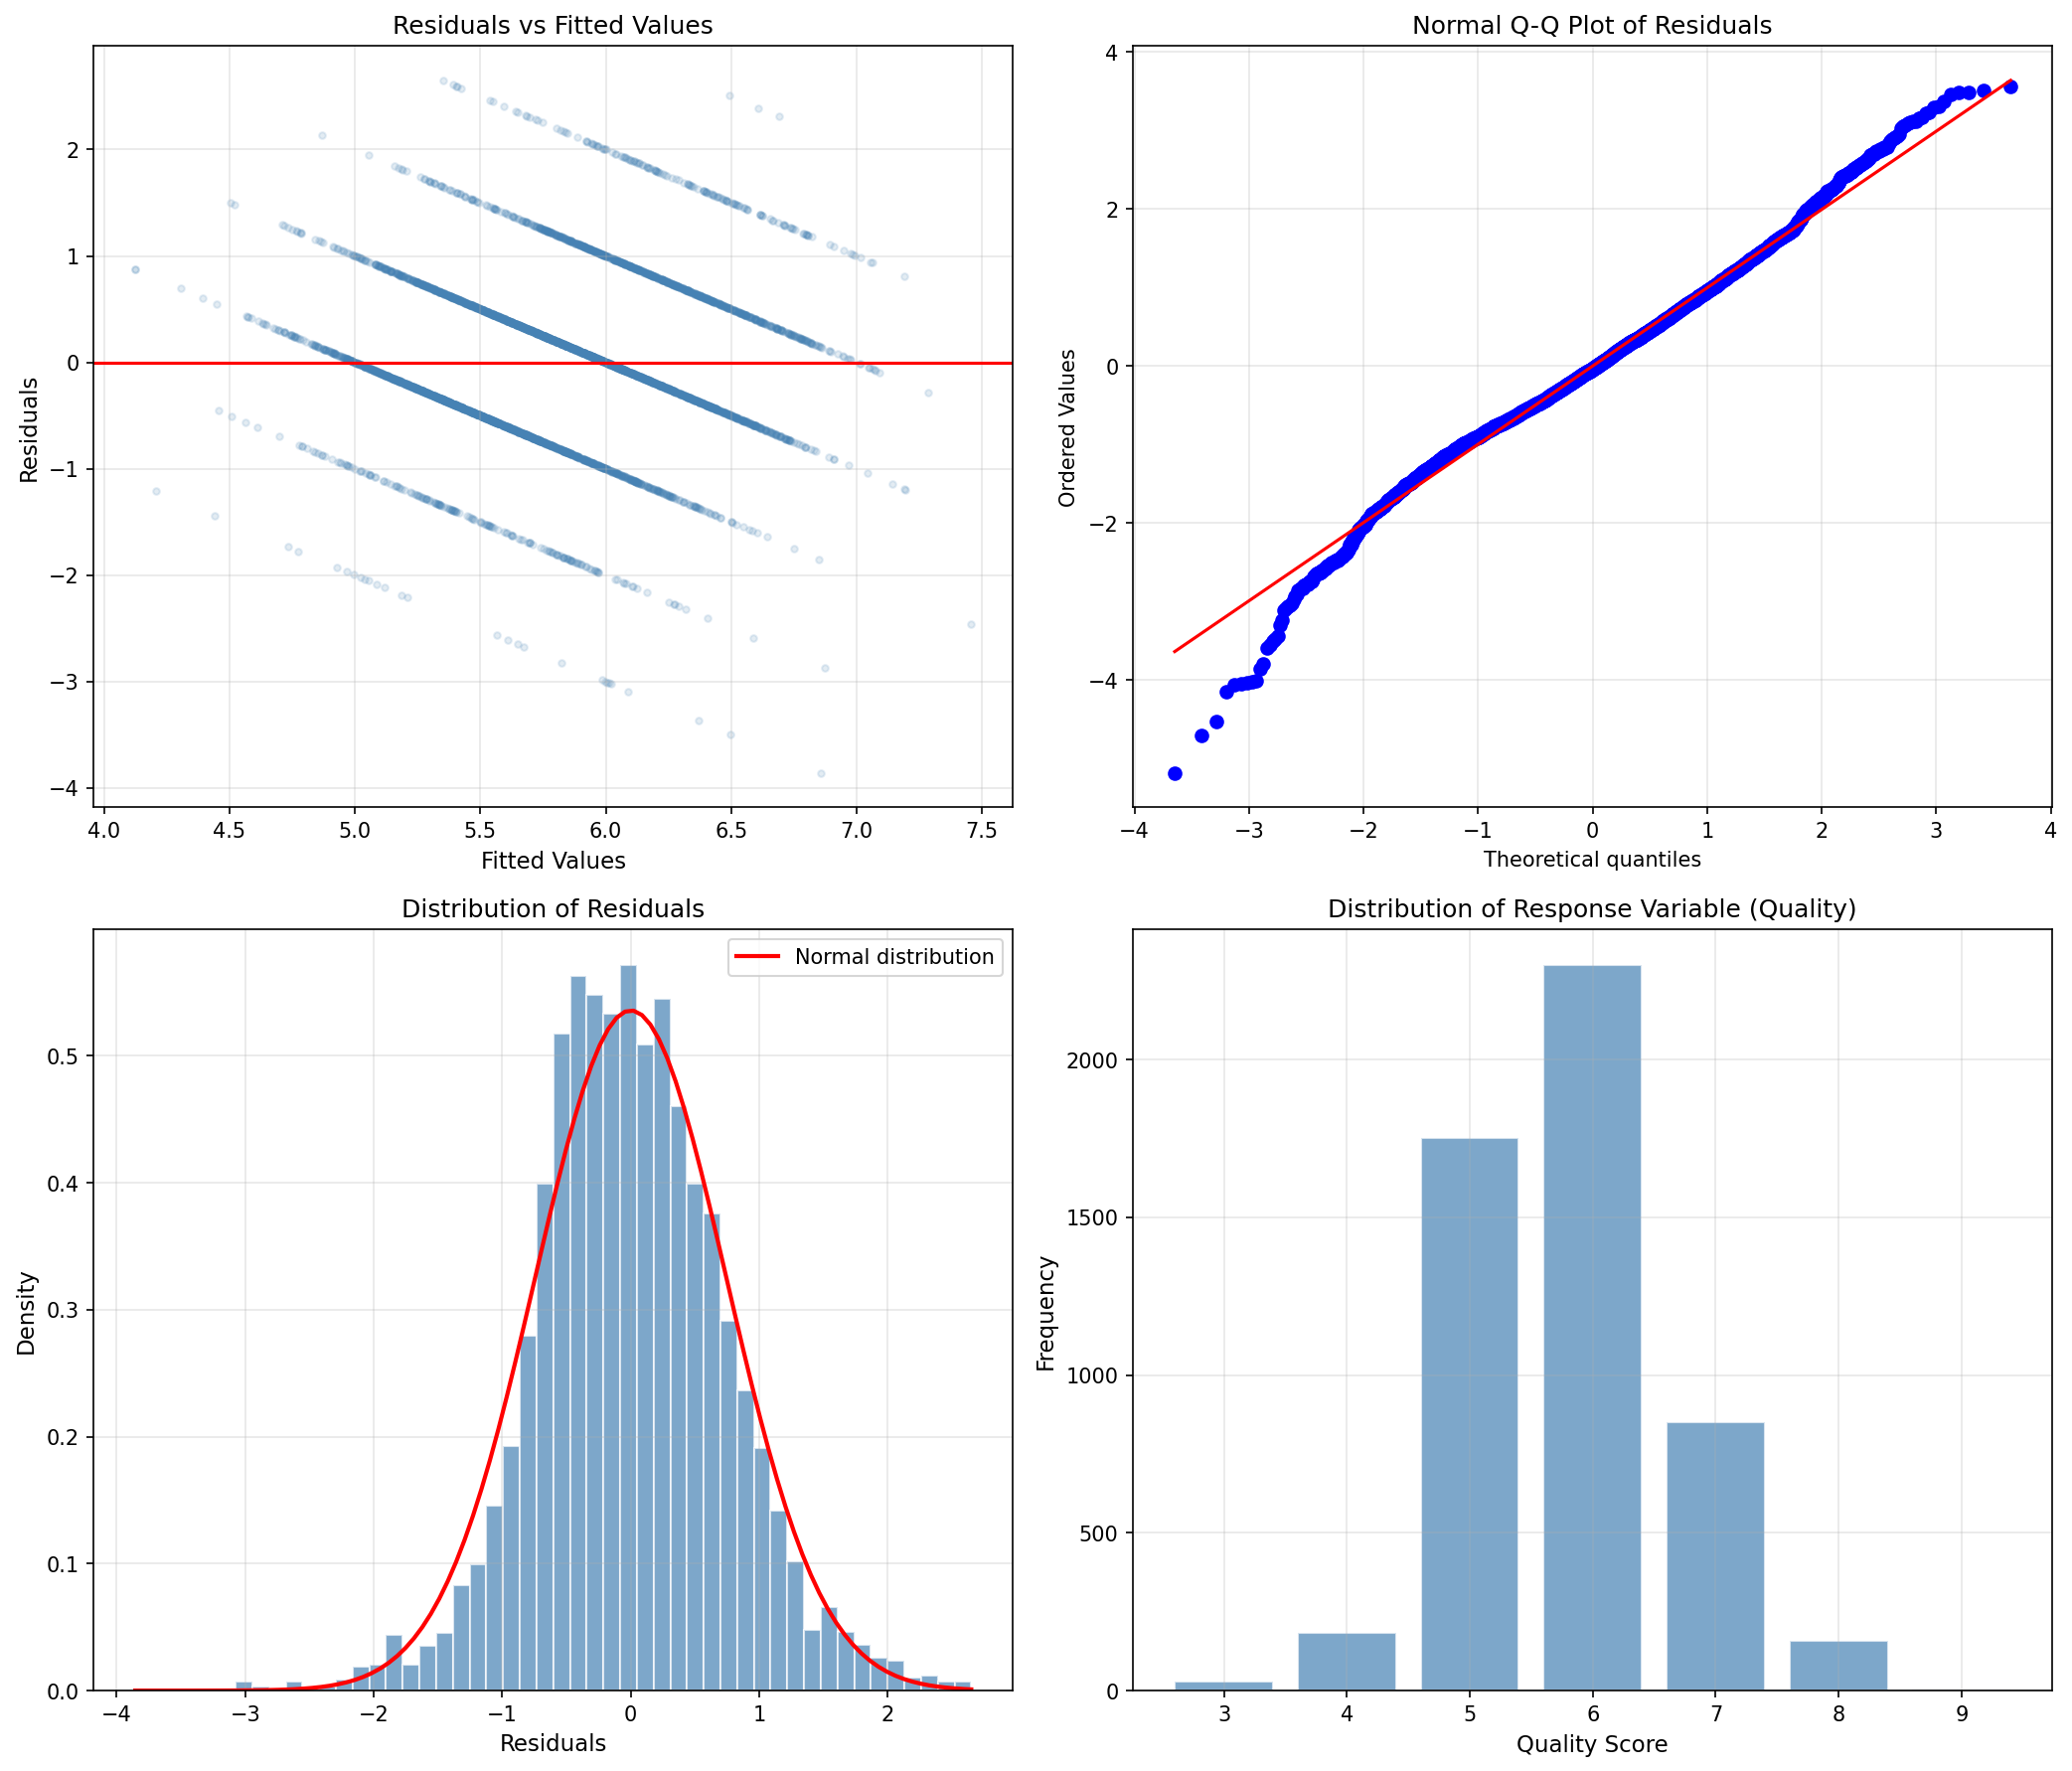
\includegraphics[width=\textwidth]{model_diagnostics.png}
    \caption{Διαγνωστικά γραφήματα: (α) υπόλοιπα vs προβλεπόμενες τιμές, (β) Q-Q plot, (γ) κατανομή υπολοίπων, (δ) κατανομή μεταβλητής απόκρισης.}
    \label{fig:diagnostics}
\end{figure}

\begin{table}[H]
\centering
\caption{Αποτελέσματα διαγνωστικών ελέγχων}
\label{tab:diagnostics}
\begin{tabular}{llll}
\toprule
\textbf{Έλεγχος} & \textbf{Στατιστική} & \textbf{p-value} & \textbf{Αποτέλεσμα} \\
\midrule
Κανονικότητα (Jarque-Bera) & $JB = 222.07$ & $6.0 \times 10^{-49}$ & Απορρίπτεται \\
Κανονικότητα (Shapiro-Wilk) & $W = 0.991$ & $4.4 \times 10^{-17}$ & Απορρίπτεται \\
Ομοσκεδαστικότητα (Breusch-Pagan) & $BP = 75.01$ & $1.4 \times 10^{-11}$ & Απορρίπτεται \\
Αυτοσυσχέτιση (Durbin-Watson) & $DW = 2.041$ & -- & Αποδεκτό \\
\bottomrule
\end{tabular}
\end{table}

\subsection{Πολυσυγγραμμικότητα (VIF)}

\begin{table}[H]
\centering
\caption{Παράγοντας πληθωρισμού διακύμανσης (VIF)}
\label{tab:vif}
\small
\begin{tabular}{lrl}
\toprule
\textbf{Μεταβλητή} & \textbf{VIF} & \textbf{Αξιολόγηση} \\
\midrule
\begin{english}fixed acidity\end{english}        & 2.70 & Αποδεκτό \\
\begin{english}volatile acidity\end{english}     & 1.85 & Αποδεκτό \\
\begin{english}citric acid\end{english}          & 1.56 & Αποδεκτό \\
\begin{english}residual sugar\end{english}       & 3.38 & Αποδεκτό \\
\begin{english}chlorides\end{english}            & 1.59 & Αποδεκτό \\
\begin{english}free sulfur dioxide\end{english}  & 2.09 & Αποδεκτό \\
\begin{english}total sulfur dioxide\end{english} & 2.79 & Αποδεκτό \\
\begin{english}density\end{english}              & 6.26 & Μέτρια πολυσυγγρ. \\
\begin{english}pH\end{english}                   & 1.70 & Αποδεκτό \\
\begin{english}sulphates\end{english}            & 1.41 & Αποδεκτό \\
\begin{english}alcohol\end{english}              & 2.53 & Αποδεκτό \\
\bottomrule
\end{tabular}
\end{table}

\subsection{Εντοπισμένα προβλήματα}

\begin{enumerate}[nosep]
    \item \textbf{Διακριτή μεταβλητή απόκρισης}: Η \texttt{quality} λαμβάνει ακέραιες τιμές (3--9), παραβιάζοντας την υπόθεση συνεχούς απόκρισης. Αυτό δημιουργεί χαρακτηριστικές λωρίδες στα υπόλοιπα.

    \item \textbf{Χαμηλή ερμηνευτική ικανότητα}: $R^2 \approx 27.7\%$ -- το μοντέλο αφήνει ανεξήγητο το 72.3\% της μεταβλητότητας.

    \item \textbf{Μη κανονικά υπόλοιπα}: Οι έλεγχοι Shapiro-Wilk και Jarque-Bera απορρίπτουν κατηγορηματικά την υπόθεση κανονικότητας.

    \item \textbf{Ετεροσκεδαστικότητα}: Ο έλεγχος Breusch-Pagan υποδεικνύει μη σταθερή διακύμανση σφαλμάτων.

    \item \textbf{Πολυσυγγραμμικότητα}: Η πυκνότητα εμφανίζει μέτρια πολυσυγγραμμικότητα ($VIF = 6.26$).

    \item \textbf{Μη γραμμικές σχέσεις}: Στατιστικά σημαντικοί πολυωνυμικοί όροι (Υποερώτημα 4).
\end{enumerate}

\subsection{Εναλλακτικές προσεγγίσεις}

\begin{itemize}[nosep]
    \item \textbf{Τακτική λογιστική παλινδρόμηση}: Κατάλληλη για τη διακριτή φύση της μεταβλητής απόκρισης.
    \item \textbf{Random Forest / Gradient Boosting}: Χειρίζονται μη γραμμικότητα και αλληλεπιδράσεις.
    \item \textbf{Ridge / LASSO παλινδρόμηση}: Αντιμετωπίζουν πολυσυγγραμμικότητα.
    \item \textbf{Παλινδρόμηση Poisson}: Κατάλληλη για δεδομένα μέτρησης.
\end{itemize}

%==========================================================================
\section{Συμπεράσματα}
%==========================================================================

\begin{enumerate}[nosep]
    \item \textbf{Απλή παλινδρόμηση}: Όλες οι 11 μεταβλητές σχετίζονται σημαντικά με την ποιότητα μεμονωμένα. Ισχυρότερος προβλέπτης: αλκοόλ ($R^2 = 0.19$).

    \item \textbf{Πολλαπλή παλινδρόμηση}: Το πλήρες μοντέλο ($R^2 = 0.277$, $F = 183.41$, $p \approx 0$) αναδεικνύει 10 σημαντικούς προβλέπτες. Το \begin{english}citric acid\end{english} δεν προσφέρει σημαντική επιπλέον πληροφορία ($p = 0.138$).

    \item \textbf{Πρόσω επιλογή}: Επιβεβαιώνει τον αποκλεισμό του \begin{english}citric acid\end{english}. Οι 3 κορυφαίες μεταβλητές (\begin{english}alcohol, volatile acidity, sulphates\end{english}) εξηγούν το 92\% της ερμηνευτικής ικανότητας.

    \item \textbf{Πολυωνυμική παλινδρόμηση}: Υπάρχουν ενδείξεις μη γραμμικότητας (κυρίως για \begin{english}chlorides\end{english}), αλλά η πρακτική βελτίωση είναι περιορισμένη.

    \item \textbf{Κριτική}: Η γραμμική παλινδρόμηση παραβιάζει αρκετές υποθέσεις (διακριτή απόκριση, μη κανονικά υπόλοιπα, ετεροσκεδαστικότητα). Εναλλακτικές μέθοδοι (τακτική λογιστική παλινδρόμηση, αλγόριθμοι μηχανικής μάθησης) θα ήταν καταλληλότερες.
\end{enumerate}

Συνολικά, παρά τους περιορισμούς, η ανάλυση αποκάλυψε ότι οι φυσικοχημικές ιδιότητες εξηγούν ένα σημαντικό αλλά μη πλήρες μέρος ($\approx 28\%$) της μεταβλητότητας στην ποιότητα κρασιού, με το αλκοόλ, την πτητική οξύτητα και τα θειικά να αποτελούν τους κυρίαρχους προβλέπτες.

\end{document}
